\noindent Mathematical models for COVID-19 have shown that the parameters values are not necessarily the same in each country. For this reason, we use data from Mexico city plus the surrounding metropolitan area to estimate some parameter values of system~\ref{model1}. These values will be used to exemplify our results. For the parameter estimation process, we fixed some parameter values according the literature, and then followed a two-stages process: i) before, and ii) after mitigation measures were implemented. In both stages, we used model~\ref{model1}, with no vaccination ($\lambda_V$ and $V = 0$). For the first stage, we consider the dates from the first day of symptoms onset reported (February 19) until March 23, 2020. For the second stage, we took a month later than mitigation measures were implemented, that is, from March 23 to April 23, 2020, and results are shown in Figure~\ref{Figure1}. It is important to stress that the second stage is used to partially represent the non-pharmaceutical interventions, which implies a reduction of contact transmission rates. Parameter values are summarized in Table~\ref{table_icparam}, while fixed parameters values are shown in Table~\ref{table_fixparam}.

%\section{Parameter setting}

%Parameter setting is done in two stages; in both stages,  we started off the model (\ref{model1}), which is simplified by adapting it to the stage to be modeled. With the parameters obtained through the adjustment, the value of the basic reproductive number ($ R_0 $) will be obtained, defined as the average number of secondary infections generated by an infectious individual, during their entire period of infectivity, when in contact with a population of fully susceptible individuals.

%For the second stage analyzed, corresponding to the quarantine period in Mexico and which includes from March 23 to May 31, 2020, we used the model (\ref{model2}) considering one more class, which corresponds to the population of people dying due to disease. Once normalized with respect to the population of living individuals, the model is given by:

%\begin{eqnarray}\label{model2}
%S'(t)&=&\mu \bar{N} -\frac{\beta_S I_S+\beta_AI_A}{\bar{N}}S-\mu S+\delta_R R %\nonumber \\
%E'(t)&=&\frac{\beta_S I_S+\beta_AI_A}{\bar{N}}S-(\mu+\delta_E) E \nonumber\\
%I'_S(t)&=&p \delta_E E-(\mu+\alpha_S) I_S\\
%I'_A(t)&=&(1-p) \delta_E E-(\mu+\alpha_A) I_A \nonumber\\
%R'(t)&=& \theta \alpha_S I_S+\alpha_A I_A-(\mu+\delta_R) R  \nonumber\\
%D'(t)&=&  (1-\theta) \alpha_S  I_S \nonumber
%\end{eqnarray}
%where $\bar{\epsilon}$ represents the reduction factor in infection rates due to the quarantine effect.

%For the model, the parameters $ \mu = 0.653 \times 10^{- 6} $ and $ \delta_E = 0.196078431 $ were set, which correspond to the reciprocals of the half-life, which is 75 years, and the estimated incubation period in 5.1 days \cite{peru2}. Now, using the next generation matrix method, the basic reproductive number for model (\ref{model2}) is given by:

%\begin{equation}\label{R02}
%R_{01}=\frac{p\delta_E\beta_S}{(\mu+\alpha_S)(\mu+\delta_E)}+\frac{(1-p)\delta_E\beta_A}{(\mu+\alpha_A)(\mu+\delta_E)},
%\end{equation}



%Using the MCMC method to estimate parameters, we have the following values and their confidence intervals for each estimated parameter.

\begin{table}[h!]
\begin{center}
    \begin{tabular}{>{\centering}p{0.2\textwidth}p{0.4\textwidth}p{0.2\textwidth}}
        \toprule
        Parameter & 95\% Confidence Interval & Quantile 50
        \\
        \midrule
        $\beta_S$ & $[\num{0.6689}, \num{1.191}]$   &  $\num{0.9303}$
        \\
        $\beta_A$ & $[\num{0.5019}, \num{0.7867}]$  &  $\num{0.6441}$
        \\
        $p$       & $[\num{0.06088}, \num{0.2239}]$ &  $\num{0.1213}$
        \\
        $\xi$     & $[\num{0.3707}, \num{0.4113}]$  & $\num{0.3905}$
        \\
      %$\mu_S$ & $1.930\times 10^{-1}$ $(9.464\times 10^{-2},3.416\times
      % 10^{-1})$ %   \\
      %$\alpha_S$ & $1.017\times 10^{-1}$ $(5.685\times 10^{-2},1.797\times
      % 10^{-1})$    \\
      %$\alpha_A$ & $1.928\times 10^{-1}$ $(1.143\times 10^{-1},3.04\times
      % 10^{-1})$  \\
      %$R_0$ & $5.385$ $(4.062,7.782)$
        \\
    \bottomrule
\end{tabular}
  \caption{Estimated values for some parameters of system~\ref{model1}.}\label{table_icparam}
\end{center}
\end{table}

%\pagebreak
\begin{table}[h!]
    \begin{center}
        \begin{tabular}{>{\centering}p{0.2\textwidth}p{0.2\textwidth}p{0.2\textwidth}}
            \toprule
            Parameter & Value & References
            \\
            \midrule
            $\delta_{E}^{-1}$ & \SI{5.1}{days}   &  \cite{Tian2020}
            \\
            $\alpha_{S}^{1}$  & \SI{5.97}{days}  &  \cite{Acuna2020}
            \\
            $\alpha_{A}^{-1}$ & \SI{10.81}{days} & \cite{Acuna2020}
            \\
            $\delta_{R}^{-1}$ & \SI{1}{years}     &
            \\
            $\mu^{-1}$        & \SI{75}{years}   &
            \\
            \bottomrule
        \end{tabular}
        \caption{
            Fixed parameters values of system~\ref{model1}.
        }
        \label{table_fixparam}
    \end{center}
\end{table}
%

Figure~\ref{Figure1} shows the fitting curves for the two time periods. With
the obtained parameters, we simulated the evolution of the number of infected
individuals starting on February 19, 2020 until July 2022. With  these dates,
it is possible to observe two outbreaks (Figure~\ref{Figure2}), where the
second one is referred to as the second wave of COVID-19. With this scenario,
it is possible to evaluate the effect of different vaccination strategies,
which we consider to start to be applied on March 2021, which is the time prior
to the onset of the second wave.
\begin{figure}[!h]
  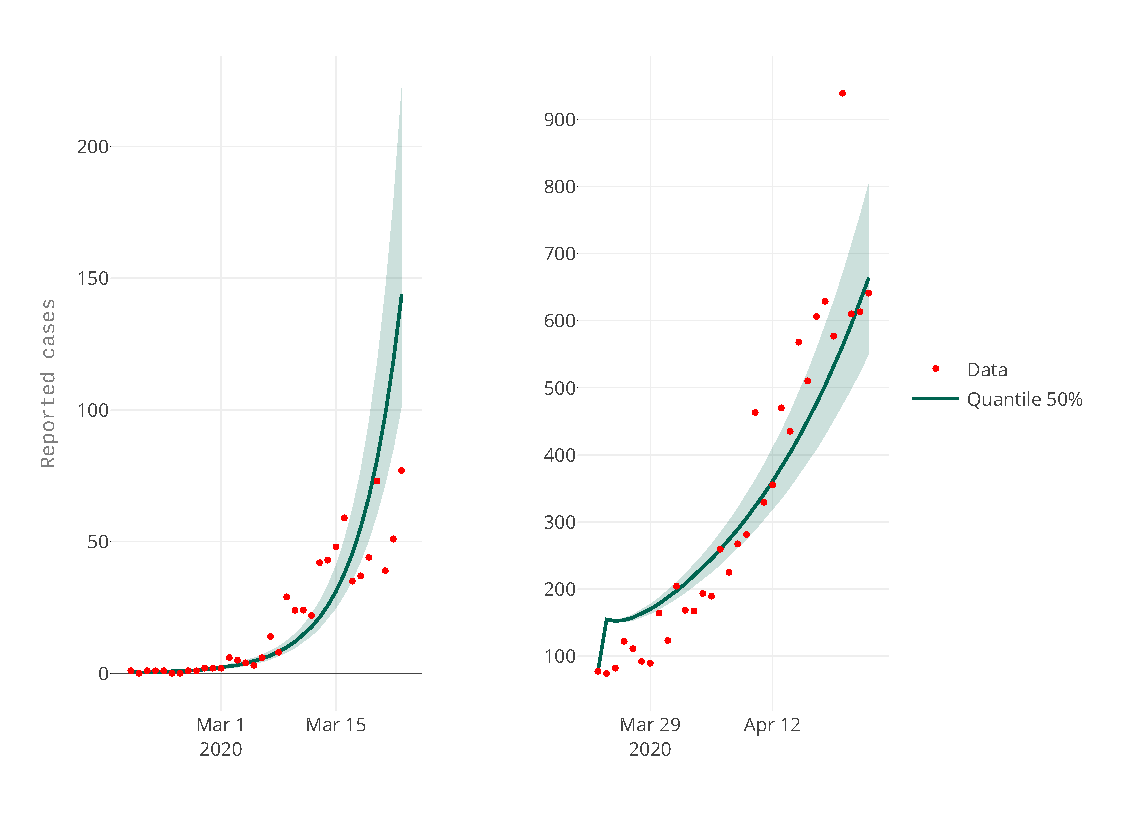
\includegraphics[width=\textwidth]{FittingCurves.eps}
  \caption{Fitting curves for the early phase of the COVID-19 outbreak in
      Mexico City plus the surrounding metropolitan area. The left side shows
      the outbreak from February 19 to March 23, 2020. The right side shows the
      outbreak from March 23 to April 23, 2020.}
  \label{Figure1}
\end{figure}
\pagebreak
\begin{figure}[!h]
  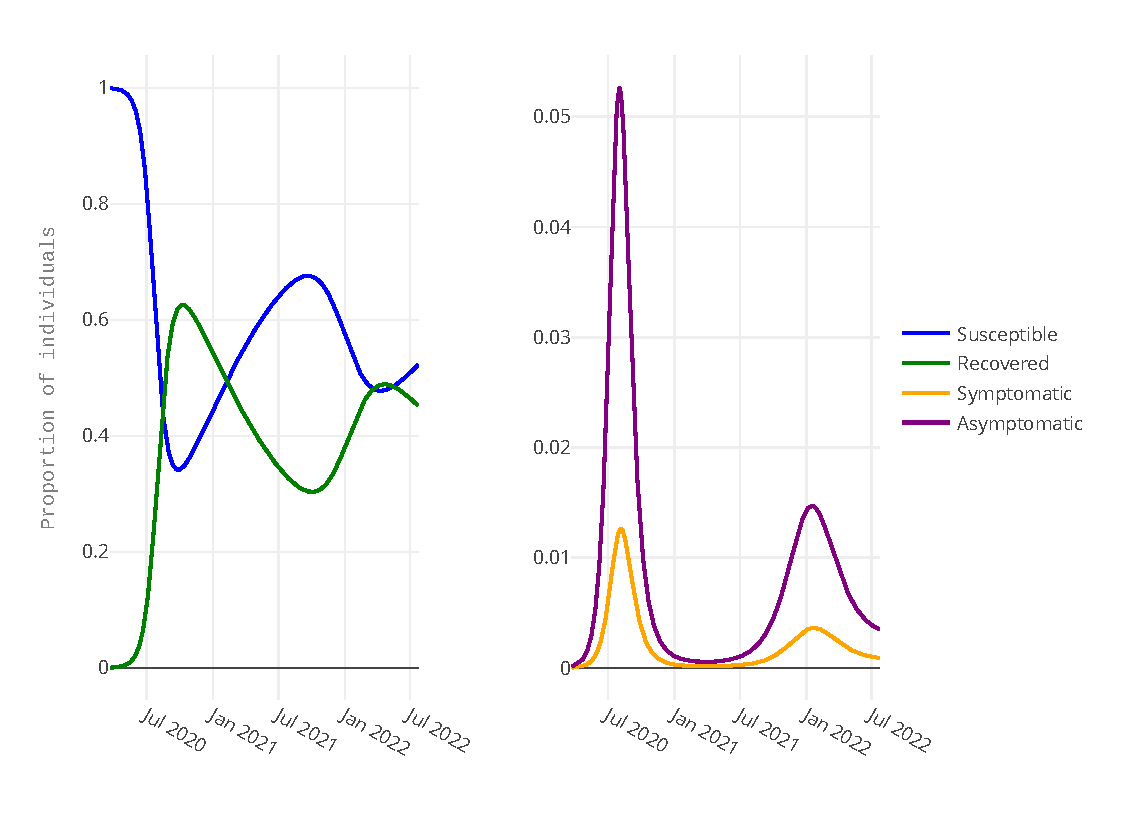
\includegraphics[width=\textwidth]{Solutions.eps}
  \caption{Dynamics populations without vaccination process. Here,
      system~\ref{model1} is reduced when considering $\lambda_V = \delta_V =
      0$, $\epsilon = 1$, and $V(0) = 0$.}
    \label{Figure2}
\end{figure}
\pagebreak